\documentclass[12pt]{article}
\usepackage{amsmath, amssymb, amsthm}    
\usepackage{parskip}  
\usepackage{enumitem}  
\usepackage{geometry}    
\usepackage{titling}     
\usepackage{color}       
\usepackage{hyperref}   
\usepackage{tipa}
\usepackage{graphicx}     
\usepackage{mathrsfs}
\usepackage{tikz}
\usepackage{tkz-euclide}

%\geometry{legalpaper, portrait, margin=1in}
%\linespread{2}
\setlength{\parindent}{3em}   
\setlength{\parskip}{1em}   
\setlength{\droptitle}{-5em}

\newcommand{\N}{\mathbb{N}}
\newcommand{\Z}{\mathbb{Z}}
\newcommand{\R}{\mathbb{R}}
\newcommand{\C}{\mathbb{C}}
\newcommand{\fc}{F^{\C}}

\newcommand{\poincare}{Poincar\'{e} }
\newcommand{\Tr}{\text{Tr}}
\newcommand{\Range}{\text{Range}}
\newcommand{\Ker}{\text{Ker}}
\newcommand{\inv}{^{-1}}
\newcommand{\Log}{\text{Log}}

\newcommand{\spceq}{\hspace{2mm} = \hspace{2mm}}
\newcommand{\ttspc}{\hspace{1mm}}
\newcommand{\ttc}{, \hspace{1mm}}


\newcommand{\lftmat}[4]{\begin{bmatrix} {#1} & {#2} \\ {#3} & {#4} \end{bmatrix}}
\newcommand{\stanlftmat}{\lftmat{a}{b}{c}{d}}
\newcommand{\pointmat}[2]{\lftmat{{#2}}{{#1}}{-1}{-{#2}}}
\newcommand{\stanpointmat}{\pointmat{x}{y}}
\newcommand{\linenoendmat}[2]{\begin{bmatrix} -{#2} & -{#1} \\ 1 & {#2} \end{bmatrix}}
\newcommand{\stanlinenoendmat}{\linenoendmat{l_1}{l_2}}
\newcommand{\lineendmat}[2]{\begin{bmatrix} -1 & -{#1} \\ 0 & 1 \end{bmatrix}}
\newcommand{\stanlineendmat}{\lineendmat{l_1}{l_2}}

\newcommand{\specialend}{(\infty^2\ttc\infty)}

% Theorem counters
\theoremstyle{plain}
\newtheorem{theorem}{Theorem}[section]
\newtheorem{definition}{Definition}[section]
\newtheorem{corollary}[theorem]{Corollary}
\newtheorem{lemma}{Lemma}[section]
\newtheorem{proposition}[theorem]{Proposition}


% Problem environments
\theoremstyle{definition}
\newtheorem{problem}[theorem]{Problem}
\newtheorem{example}[definition]{Example}


\title{Fixing Heinrich Guggenheimer's Fucking Wild Notation and Generally Shitty/Vague Paper}
%\title{The Hyperbolic Geometry of Linear Fractional Transformations in Complexified Fields}
\author{Anna Blinderman, Logan Goldberg}
\date{}

\begin{document}

\maketitle

\newcommand{\wtftitle}[1]{\noindent\begin{Large}\textbf{{#1}}\end{Large}\vspace{3mm}}
\newcommand{\wtftheorem}[1]{\noindent\textbf{{#1}}. \hspace{1mm}}
\newcommand{\wtfqed}{\vspace{-5mm}\begin{flushright} \qedsymbol \end{flushright}}








\wtftitle{Abstract}

In his paper \textit{The Hilbert Model of Hyperbolic Geometry}, Heinrich Guggenheimer classifies linear fractional transformations with coefficients in a real, ordered field $F$ into point reflections and two types of line reflections in the context of hyperbolic geometry. In this paper we first introduce a clear notation for such transformations and attempt to motivate the algebra behind Guggenheimer's classifications. We then choose the real ordered field $F = \R$ and illustrate various transformations in $F$ using the \poincare disk model for hyperbolic geometry. Motivated by Guggenheimer's claim that this geometry can be developed similarly for transformations with coefficients in $\fc$ (the complexified\footnote{See appendix.} version of $F$), we attempt to do so for $\R^{\C}$ (i.e. $\C$). 








\[\]\wtftitle{Introduction}

To understand hyperbolic geometry, we must consider Euclid's five postulates, which make up the axiomatic structure (??) of Euclidean geometry [phrasing of this whole damn sentence...]. The first four are as follows: \href{http://mathworld.wolfram.com/EuclidsPostulates.html}{[source]} [\href{https://pdfs.semanticscholar.org/ed0e/d1fee9bbe60b24be373ac1207d17ecb90b4a.pdf}{source}]
\begin{enumerate}[leftmargin = 4em, itemsep=-.8em]
	\item A straight line segment can be drawn joining any two points.
	\item Any straight line segment can be extended indefinitely in a straight line.
	\item Given any straight line segment, a circle can be drawn having the segment as radius and one endpoint as center.
	\item All right angles are congruent.
\end{enumerate}
These four postulates hold in hyperbolic geometry. However, the fifth postulate, 
\begin{enumerate}[leftmargin = 4em, itemsep=-1em]
	\setcounter{enumi}{4}
	\item If a straight line, which intersects two straight lines, form interior angles on the same side, smaller than two right angles, then these straight lines, extended to infinite, will intersect on the side where the interior angles are less than two right angles.
\end{enumerate}
is replaced with its negation: ``Through an exterior point to a straight line we can construct an infinite number of parallels to that straight line." \href{https://pdfs.semanticscholar.org/ed0e/d1fee9bbe60b24be373ac1207d17ecb90b4a.pdf}{[source]}.



Henri \poincare put forth two models for hyperbolic geometry: the \poincare half-plane and the \poincare disk. We focus here on the \poincare disk model. The set of points in the model are given by $D = \{(x\ttc y): x^2 + y^2 < 1\}$ \href{http://math2.uncc.edu/~frothe/3181alllhyp1_7.pdf}{[source]}. Lines are given by arcs of circles that are orthogonal to the boundary of the disk (does a diameter fall into this category because generalized circles or whatever? For example, the minor arc $AB$ of circle $C$ pictured below is a hyperbolic line in the \poincare disk realized by circle $O$.

\begin{tikzpicture}
\draw (0,0) circle (2.2cm);
\draw (-1.85,1.85) circle (1.41cm);
\draw[fill=black] (0,0) circle (0.05) node[right] {$O$};
\draw[fill=black] (-1.85,1.85) circle (0.05) node[left] {$C$};
\draw[fill=black] (-2.15,.48) circle (0.05) node[below right] {$A$};
\draw[fill=black] (-.48,2.15) circle (0.05) node[above right] {$B$};
(-2.15,.48)
\draw (-2.3,.35)  -- (-2.26,.5);
\draw (-2.3,.35)  -- (-2.18,.32);
%wtf add actual right angles and make the arc part bold?
\end{tikzpicture}
	
Please see the appendix ??? for further information on the \poincare disk model, namely its distance metric and the transformation we use to place points from $R^2$ into the \poincare disk.





	
\[\]\wtftitle{Notation}
	
We will first set forth the notation we will use throughout our paper. In general, we will denote the coordinates of points corresponding to point reflections as $(x \ttc y) \ttc (x' \ttc y')$, etc. As discussed later, such points will be in the interior of our \poincare disk. On the other hand, points defining lines (which lie outside of the \poincare disk) will be denoted $(l_1 \ttc l_2) \ttc (l_1' \ttc l_2')$, etc. We will then discuss general linear fractional transformations, point reflections, and two types of line reflections both algebraically and with the aid of the \poincare disk model. We first begin with an arbitrary field $F$ with the property that every positive $x \in F$ has a square root. We define the group of hyperbolic transformations over $F$ to be those linear fractional transformations\footnote{Cite class notes about this being a group} given by
\begin{equation} 
	z \mapsto \frac{az+b}{cz+d} \text{ where } z \in \C, \hspace{2mm} a \ttc b \ttc c \ttc d \in F \text{ and } ad-bc \neq 0. 
\end{equation}
For convenience, we will encode our transformations of the above form into matrices
\begin{equation}
	\lambda \stanlftmat \text{ where } \lambda \ttc a \ttc b \ttc c \ttc d \in F \text{ and } \lambda \neq 0. 
\end{equation}

It should be explicitly noted that these matrices are used only to encode our transformations\footnote{``See appendix" or something}. That is, to ``apply" a transformation encoded the matrix in (2) to a point $z_0 \in \C$, we mean that we will apply a corresponding linear fractional transformation $f$ defined by (1) to the point $z_0$. 

Because all linear fractional transformations we will use are of the form given in (2), whenever we say ``matrix" we are referring to a $2 \times 2$ matrix. 

Later we will be associating points with point reflections and lines with line reflections. In order to distinguish these geometric objects from their corresponding reflections, we will write $f_P(P_0)$ to mean the point reflection of the point $P_0$ over a point $P$ via the point reflection $f_P$ and $f_l(P_0)$ to be the line reflection of point $P_0$ over the line $l$ via the line reflection $f_l$. In a similar vein, we define $M_P$ and $M_l$ to be a matrix representation of a point reflection about $P$ and a line reflection about $l$ respectively. We will associate each point reflection with a unique point in the disk\footnote{How exactly does this ``unique association" work? }. 

Finally, we will discuss two types of line reflections: ones passing through the end $(\infty, \infty^2)$\footnote{see wherever} and ones not passing through this end. Throughout, the line to which we will refer passes through this end if and only if we explicitly specify that it does so (that is, if we simply say ``line reflection," then this line does not pass through the end $(\infty, \infty^2)$).








\[\]\wtftitle{What this Guggenheimer asshole did}
%\[\]\wtftitle{What this Guggenheimer fellow did}

We now go forth to discuss hyperbolic point reflections and hyperbolic line reflections as laid out in Guggenheimer's paper, adding motivation and further explanation wherever possible. 

Let $F$ be some real, ordered field. The coefficients of our linear fractional transformations will come from $F$.

Inspired by Euclidean geometry, we begin with the notion that both types of reflections should be of order two. That is, we want the composition of a transformation upon itself to yield the identity transformation. 

\wtftheorem{Theorem} If $M$ is a matrix encoding some linear fractional transformation $f$, then $f$ is of order two if and only if $\Tr(M) = 0$ or $M \in \lambda I$ [LOGAN: what do you want for coset notation here?]

\wtftheorem{Proof} Let $M$ be a matrix that encodes a linear fractional transformation of order two. We then must have that $M^2 = \lambda I$ for some constant $\lambda \in F$\footnote{That is, $\lambda I$ is some member of the coset containing the identity.}, where $I$ is the usual $2 \times 2$ identity matrix. In this case, we want to have that 
	\[
		\stanlftmat \stanlftmat = \lambda \lftmat{1}{0}{0}{1}
	\]
for some $\lambda \in F$. Expanding this further, we see that we must have 
	\[
		\lftmat{a^2 + bc}{b(a+d)}{c(a+d)}{bc+d^2} =  \lftmat{\lambda}{0}{0}{\lambda}
	\]
Looking at the upper-right and lower-left entries in these matrices, we see that $M^2 = \lambda I$ can hold if $a + d = 0$ or if $b = c = 0$ and $a^2 = d^2$. [LOGAN: this doesn't mean that it's $\lambda I$ since we can have $a^2 = d^2$ but not $a = d$...] Thus, since $a = d$ implies that $\Tr(M) = 0$ by definition, our theorem is proved.\wtfqed

Now, recall by equation (1) that no linear fractional transformation can be encoded in a matrix with determinant 0 since linear fractional transformations with $ad - bc = 0$ do not have inverses. Thus we may only work with matrices whose determinants are either positive or negative. We (Guggenheimer?) decide that we will encode point reflections in matrices with positive determinant and line reflections in matrices with negative determinant. 


Let $(x \ttc y)$ be a point in the \poincare disk. Then, for the matrix encoding the hyperbolic point reflection over $(x \ttc y)$ to satisfy $\Tr(M)$ and $\det M = -(y^2 - x) > 0$, we say that $M$ is of the form
\begin{equation} 
	\lambda \stanpointmat \text{ where } \lambda \in F \text{ and } x > y^2. 
\end{equation}	
As mentioned, we choose to associate each point reflection with a unique point in the disk. It follows that our points are given uniquely by $(x \ttc y) \in F^2$ inside the convex domain of the parabola $x = y^2$.

To be clear, we are not mapping this parabola to the unit disk. Similarly, we are neither mapping the points within the parabola to those in the \poincare disk nor those outside the parabola to outside the disk. Rather, we are classifying the points in $F^2$ into three disjoint subsets: those that will be in the interior of the \poincare disk (those in the convex domain defined by the parabola $x = y^2$, those that will be on the \poincare disk itself (those on the parabola $x = y^2$), and those that will be outside of the \poincare disk (those neither inside nor on the parabola $x = y^2$). 

Next, we define $F_*$ to be the extension of $F$ by $\infty$ as usual\footnote{Elaborate in the appendix}. We define an end of our geometry to be the points on our parabola, namely those pairs $(x \ttc y) \in F_*^2$ where $y = x^2$. The end $\specialend$ is of particular interest to us in our classification of line reflections. In particular, the reflection over a line $l$ given by $(l_1\ttc l_2)$ that does not pass through the end $\specialend$ can be encoded in the matrix
\[\stanlinenoendmat\]
If the line $l$ given by $(l_1\ttc l_2)$ does pass through the end $\specialend$, then the reflection over $l$ can be given by the following matrix:
\[
	\stanlineendmat
\]

Just as we uniquely associated all points with their reflections, we will uniquely associate all lines $l$ with their reflections.


\wtftheorem{Theorem} The equation of a line not passing through the end $\specialend$ must be of the form \begin{equation}
	x - 2l_2y + l_1  = 0
\end{equation} 

\wtftheorem{Proof} Notice that if a point $P$ is on a line $l$, then the reflection of $P$ over $l$ will have no effect. Regarding our point $P$ and line $l$ as their respective reflections, we then have that $f_l(P) = P$. For the same reason\footnote{presumably...}, we have that $M_l M_P M_l\inv = M_P$, whence $M_l M_P = M_P M_l$. We will first consider this in terms of matrices for lines not passing through the end $\specialend$. We have the following\footnote{$M_l M_P$ is a representative of $M_P M_l$, hence the $\lambda$}:
\begin{equation} 
\stanlinenoendmat\stanpointmat \spceq \lambda \stanpointmat\stanlinenoendmat
\end{equation}	
Expanding, we see that we must have
	\[
		\lftmat{-l_2y+l_1}{-l_2x+l_1y}{y-l_2}{x-l_2y} \spceq \lambda \lftmat{-l_2y+x}{-l_1y+l_2x}{l_2-y}{l_1-l_2y}
	\]
Looking at the lower-left corner of our matrices, we see that we must have $\lambda = -1$ since $y - l_2 = -1(l_2 - y)$. If we then consider the upper-left corner, we must have that $-l_2y + l_1 = -1(-l_2y + x)$. Simplifying, we see that equations of lines not passing through the end $\specialend$ must be of the form $x - 2l_2y + l_1  = 0$ as desired.




\wtftheorem{Theorem} The equation of a line passing through the end $\specialend$ must be of the form 
\begin{equation}
	2y = l_1
\end{equation} 

\wtftheorem{Proof} Now, if $l$ is a line passing through the end $\specialend$ and $P$ is some point on $l$, we again have that $M_l M_P = M_P M_l$. Again realizing this in terms of matrices, we have that 
\begin{equation} 
	\stanlineendmat\stanpointmat \spceq \lambda \stanpointmat\stanlineendmat
\end{equation}	
We again expand to see that 
	\[
		\lftmat{-y+l_1}{-x+l_1y}{-1}{-y} \spceq \lambda \lftmat{-y}{-l_1y+x}{1}{l_1-y}
	\]
By considering the lower-left entry into these matrices we see that $\lambda = -1$. We can now find the general form of such lines by seeing from the upper-left entries that $-y+l_1 = -y$. Simplified, our form is $2y = l_1$. 

With this in hand, we go forth to develop and visualize examples of these transformations with coefficients in the real ordered field $\R$.






\newpage\wtftitle{Examples in $\R$}

We choose $\R$ to be our real, ordered field as called for in Guggenheimer's paper and go forth to visualize some examples of transformations in the \poincare disk. We work with two triangles and two points about which each of them will be reflected\footnote{See Appendix ?? for the coode}. Triangle $T_1$ is given by the points $A_1 = 0 + 0i$, $B_1 = 1 + 0i$, and $C_1 = 0 + 1i$. Triangle $T_2$ is given by the points $A_2 = 3 + 5i$, $B_2 = -4 + 4i$, and $C_2 = 2 - 2i$. The points about which we will perform our reflections are $X = (2, 1)$ and $Y = (2, -1)$.

\iffalse
[LOGAN: change the notation to match]
\begin{tabular}{cc}
 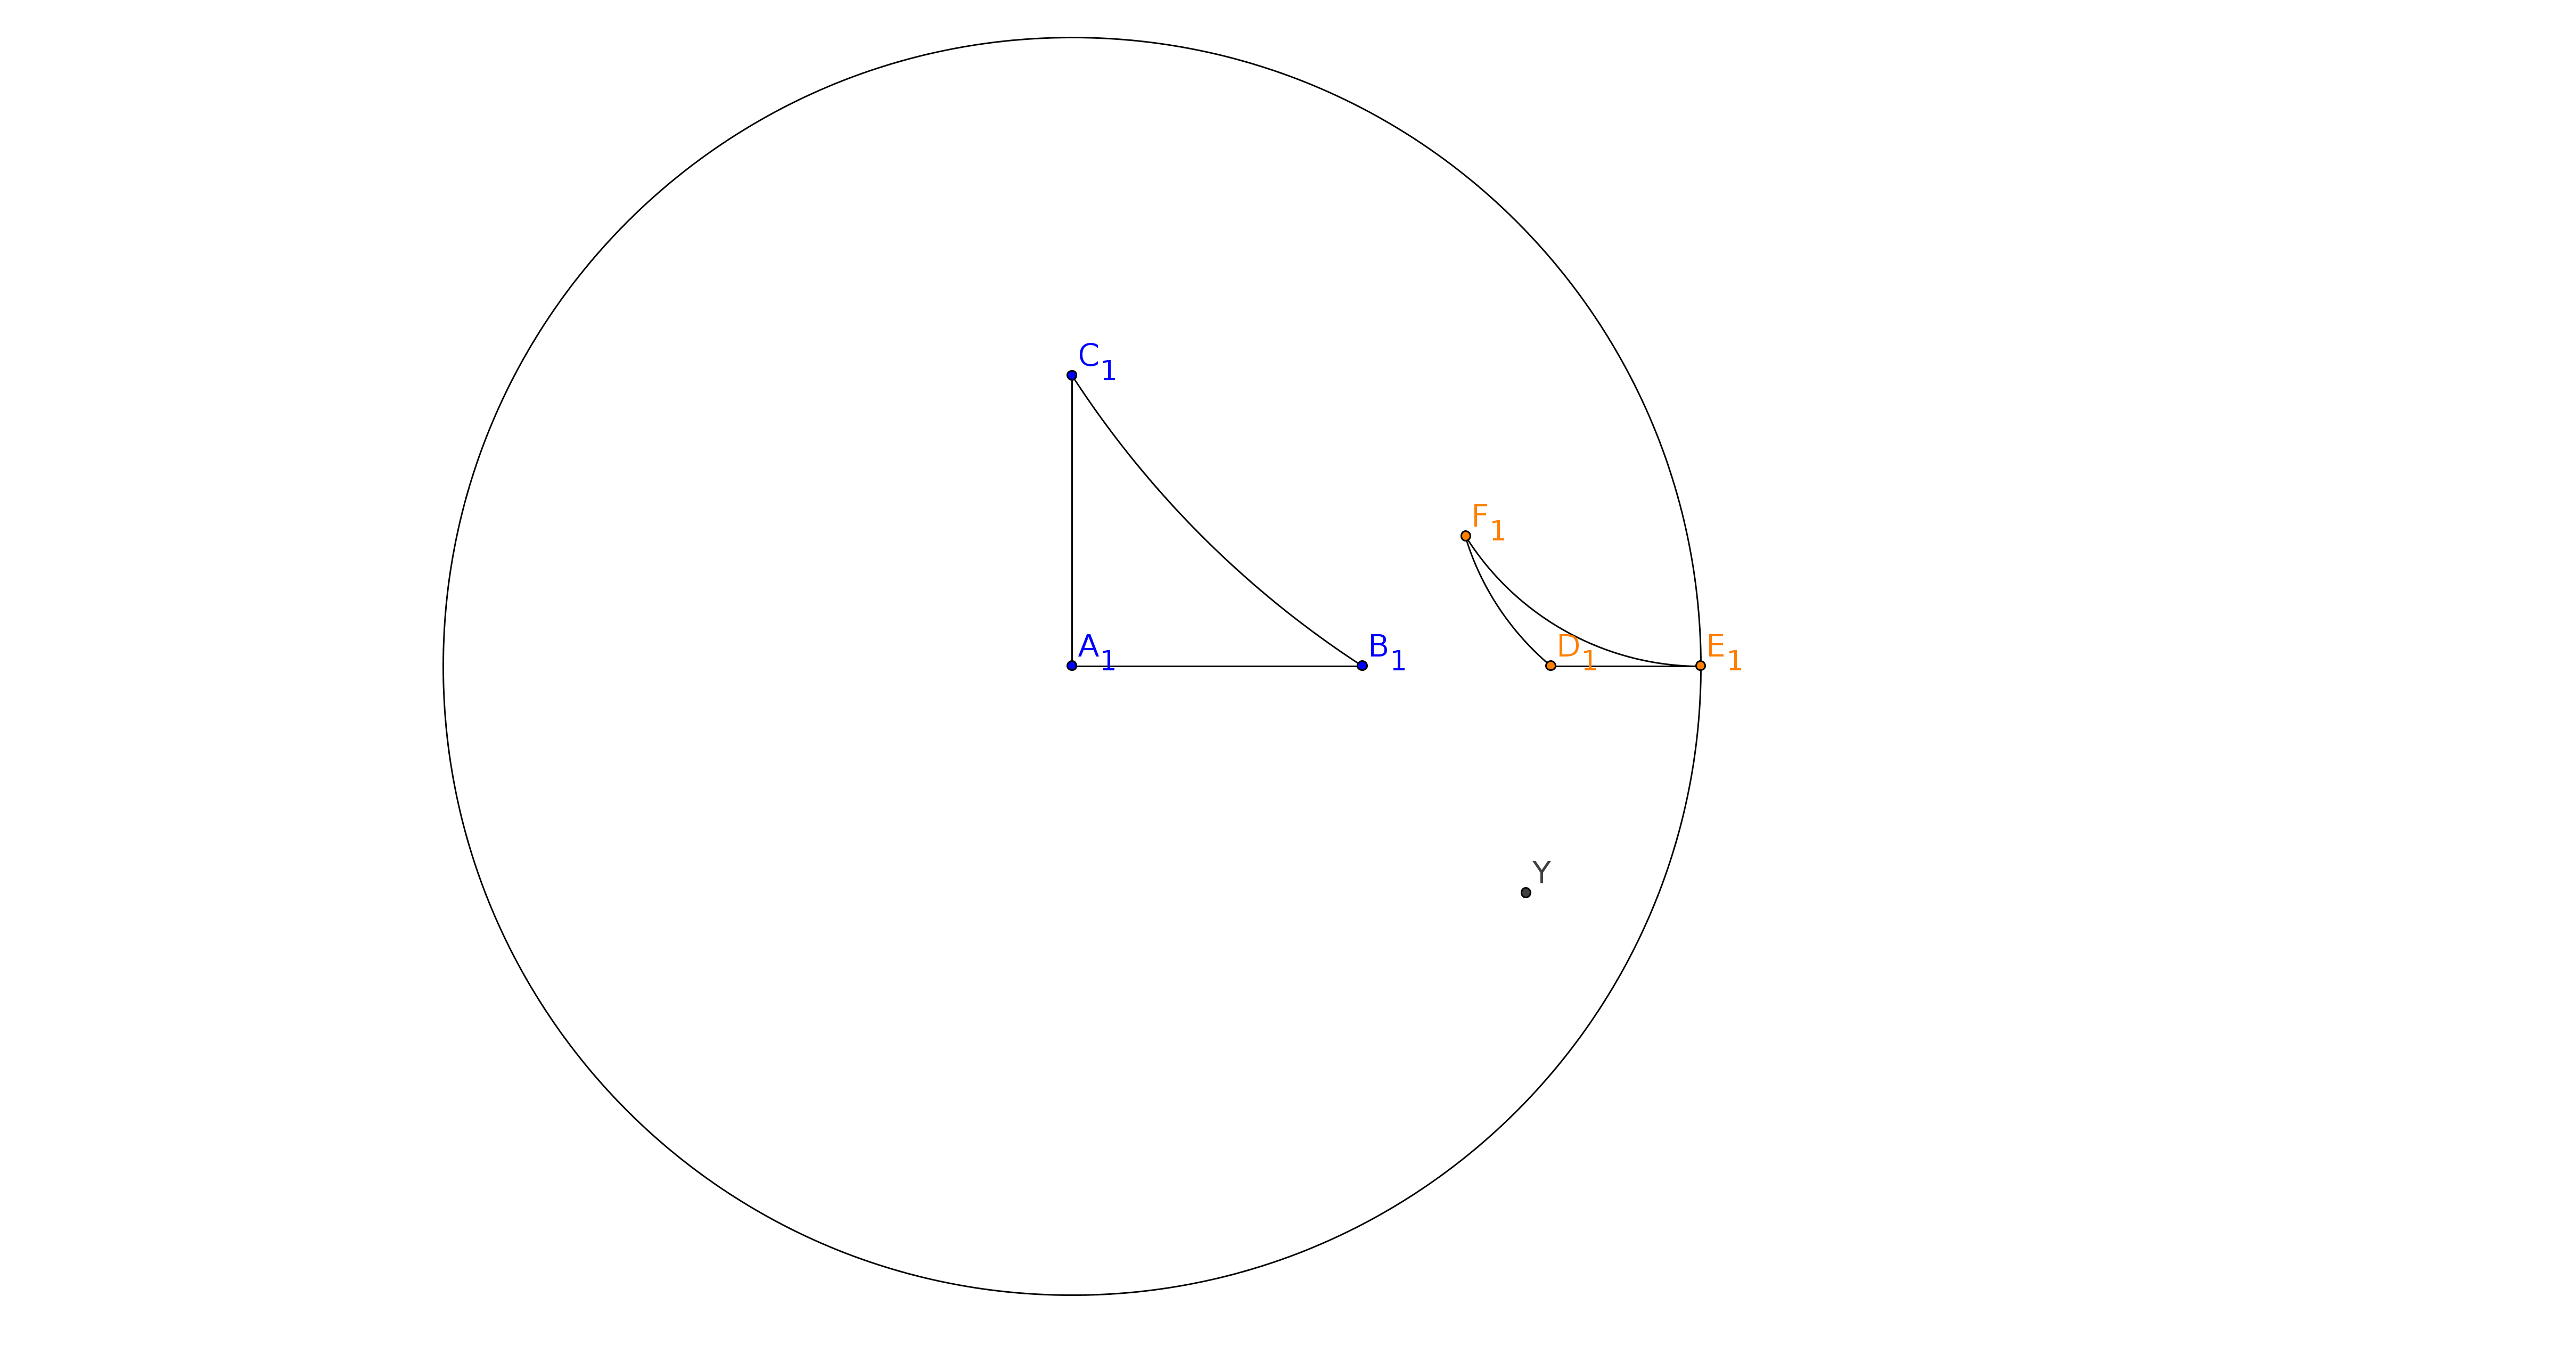
\includegraphics[width=65mm]{../images/triangle-1-point-reflection-2--1.png} & 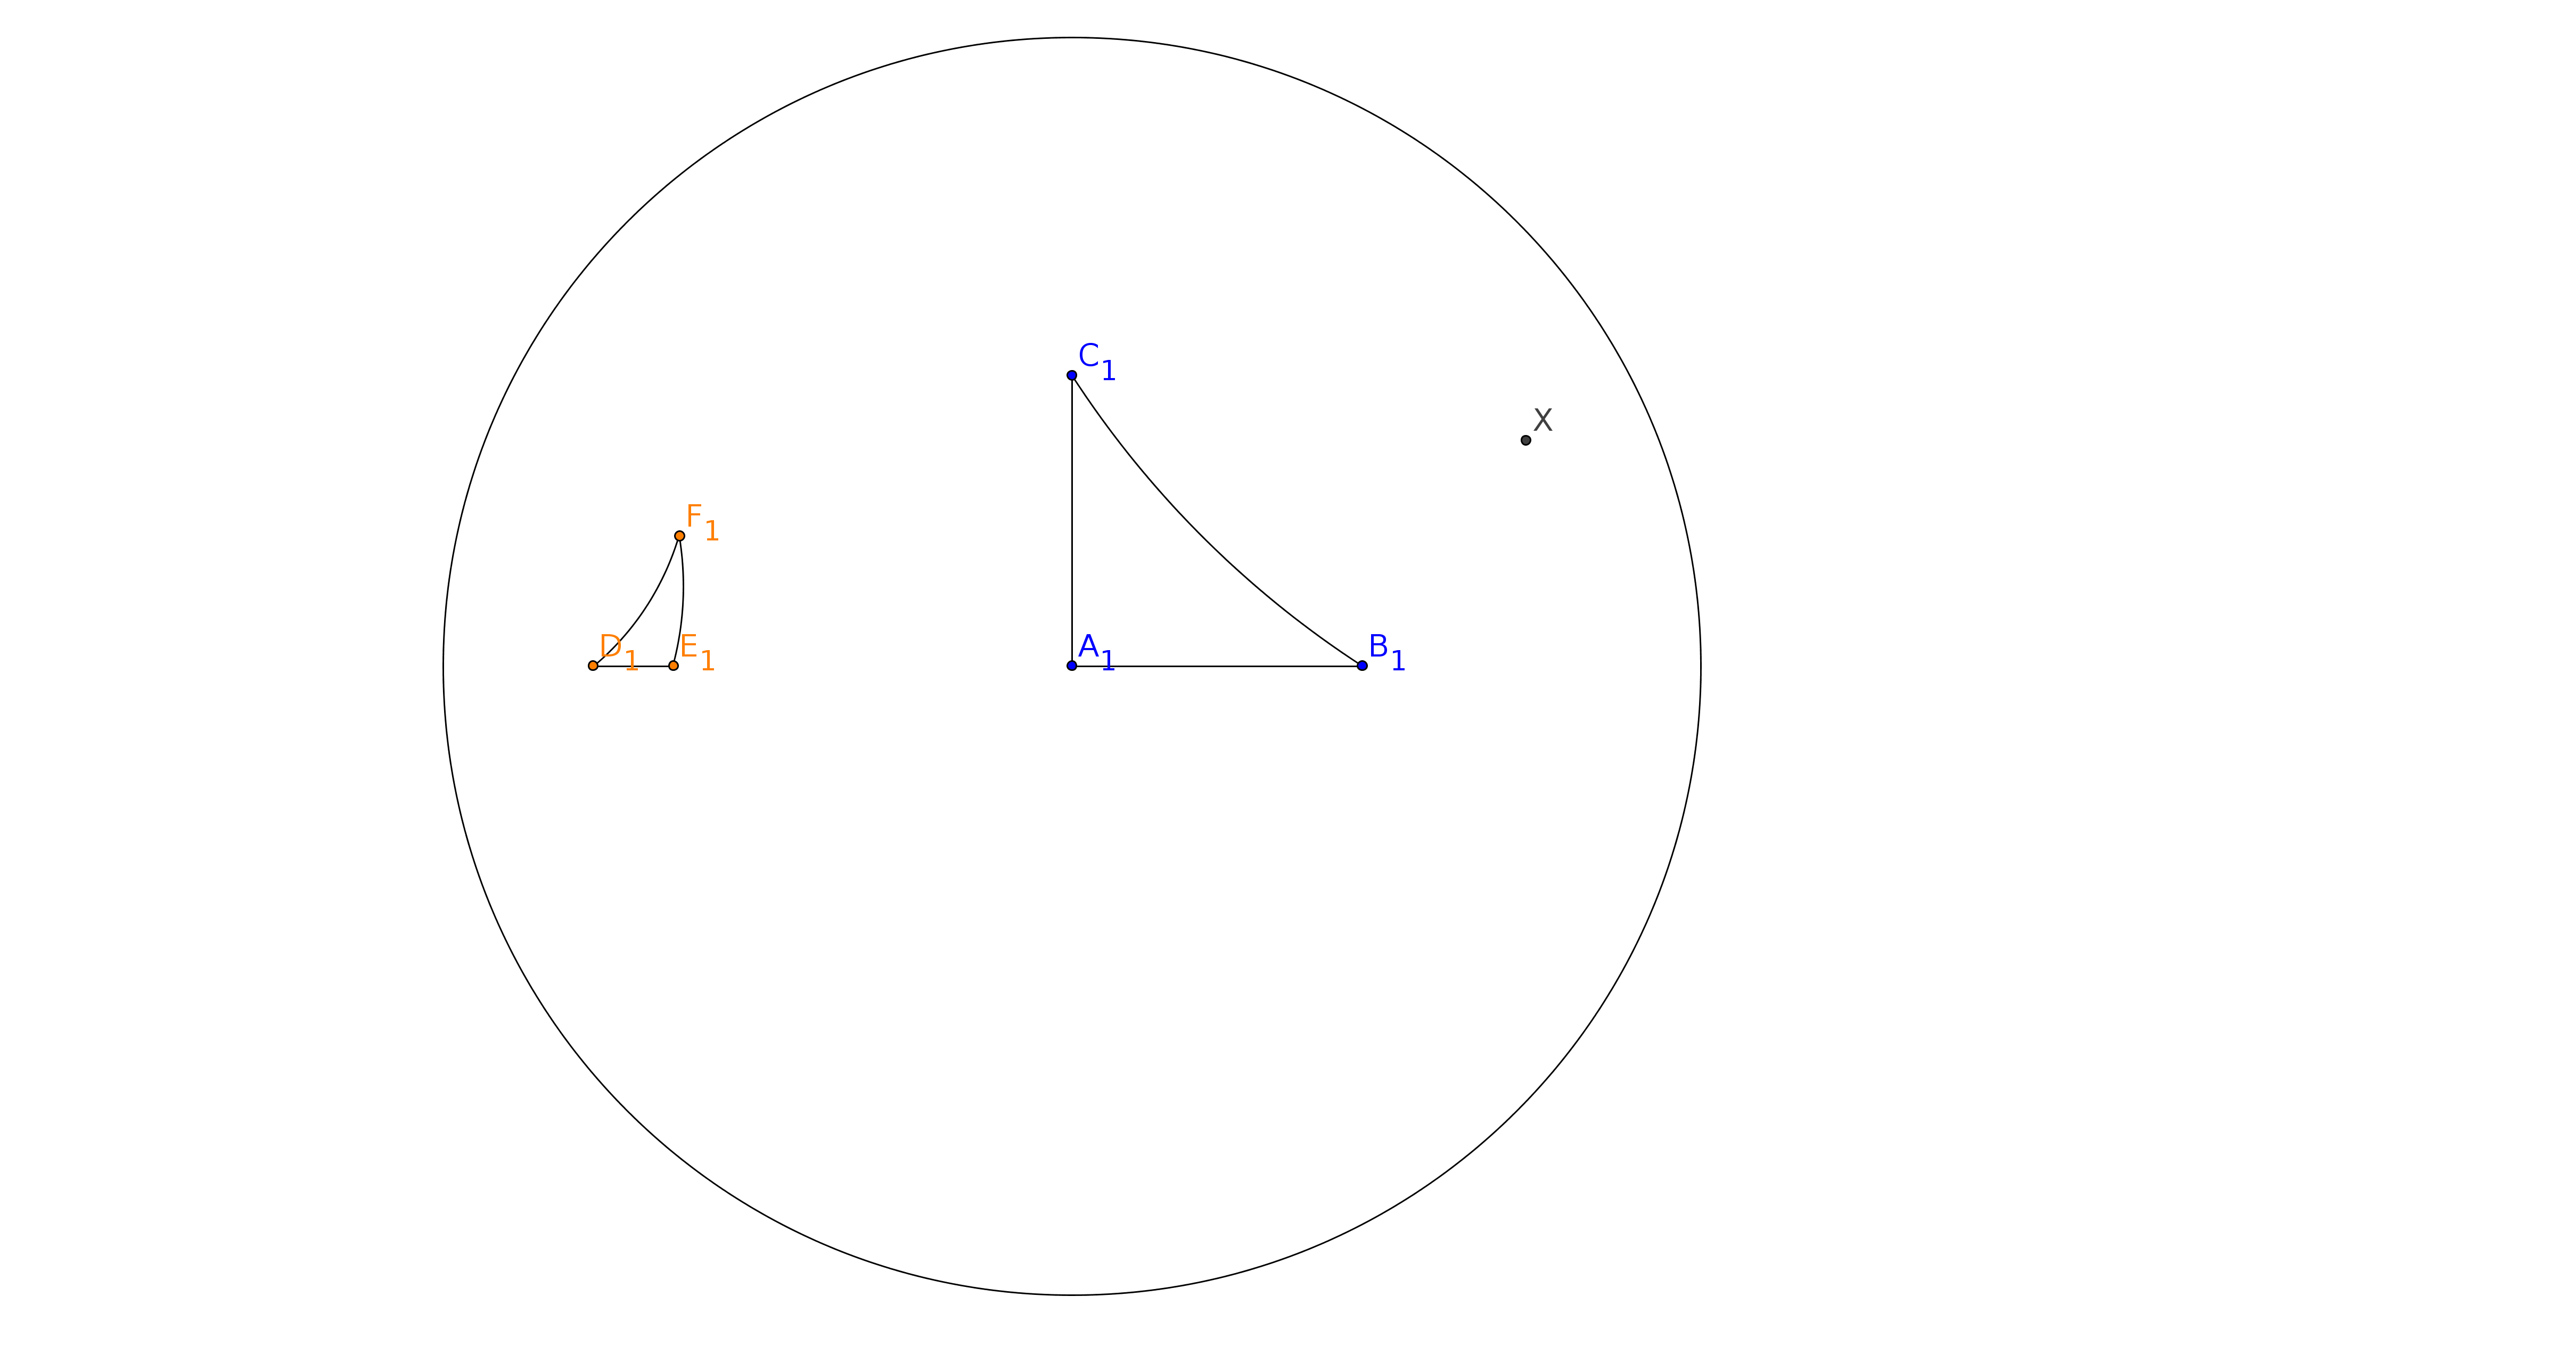
\includegraphics[width=65mm]{../images/triangle-1-point-reflection-2-1.png} \\
Triangle $T_1$ over point $X$ & Triangle $T_1$ over point $Y$  \\
& \\
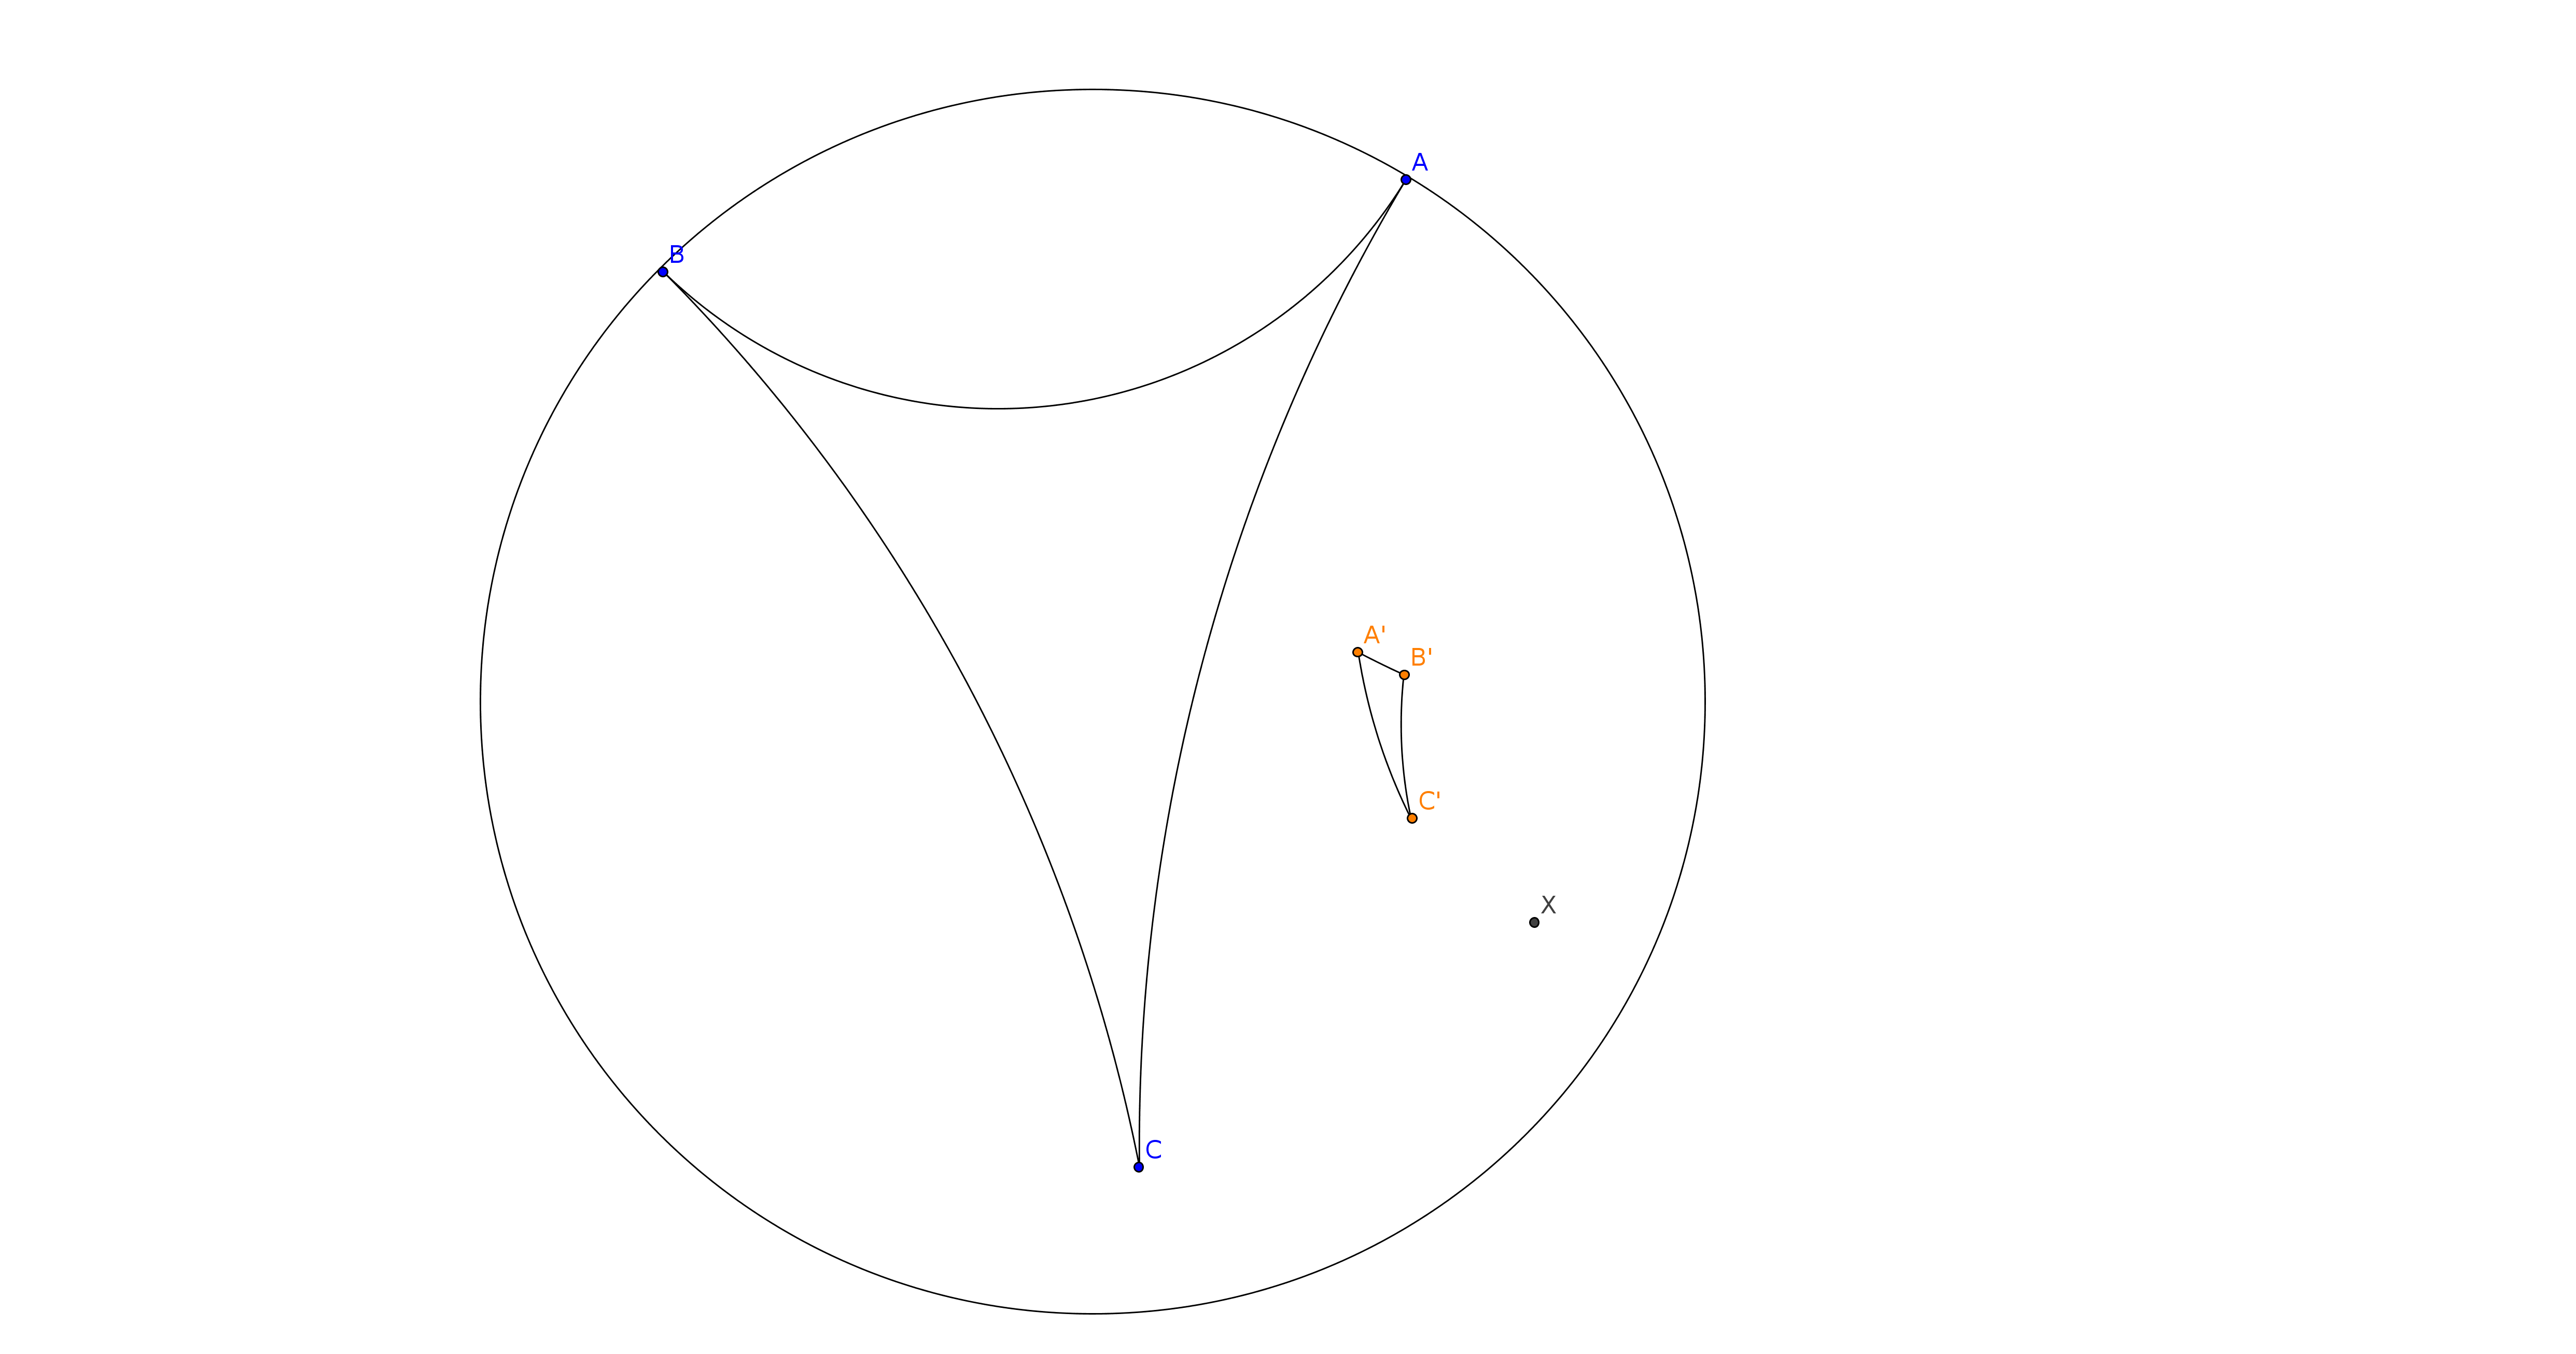
\includegraphics[width=65mm]{../images/triangle-2-point-reflection-2--1.png} & 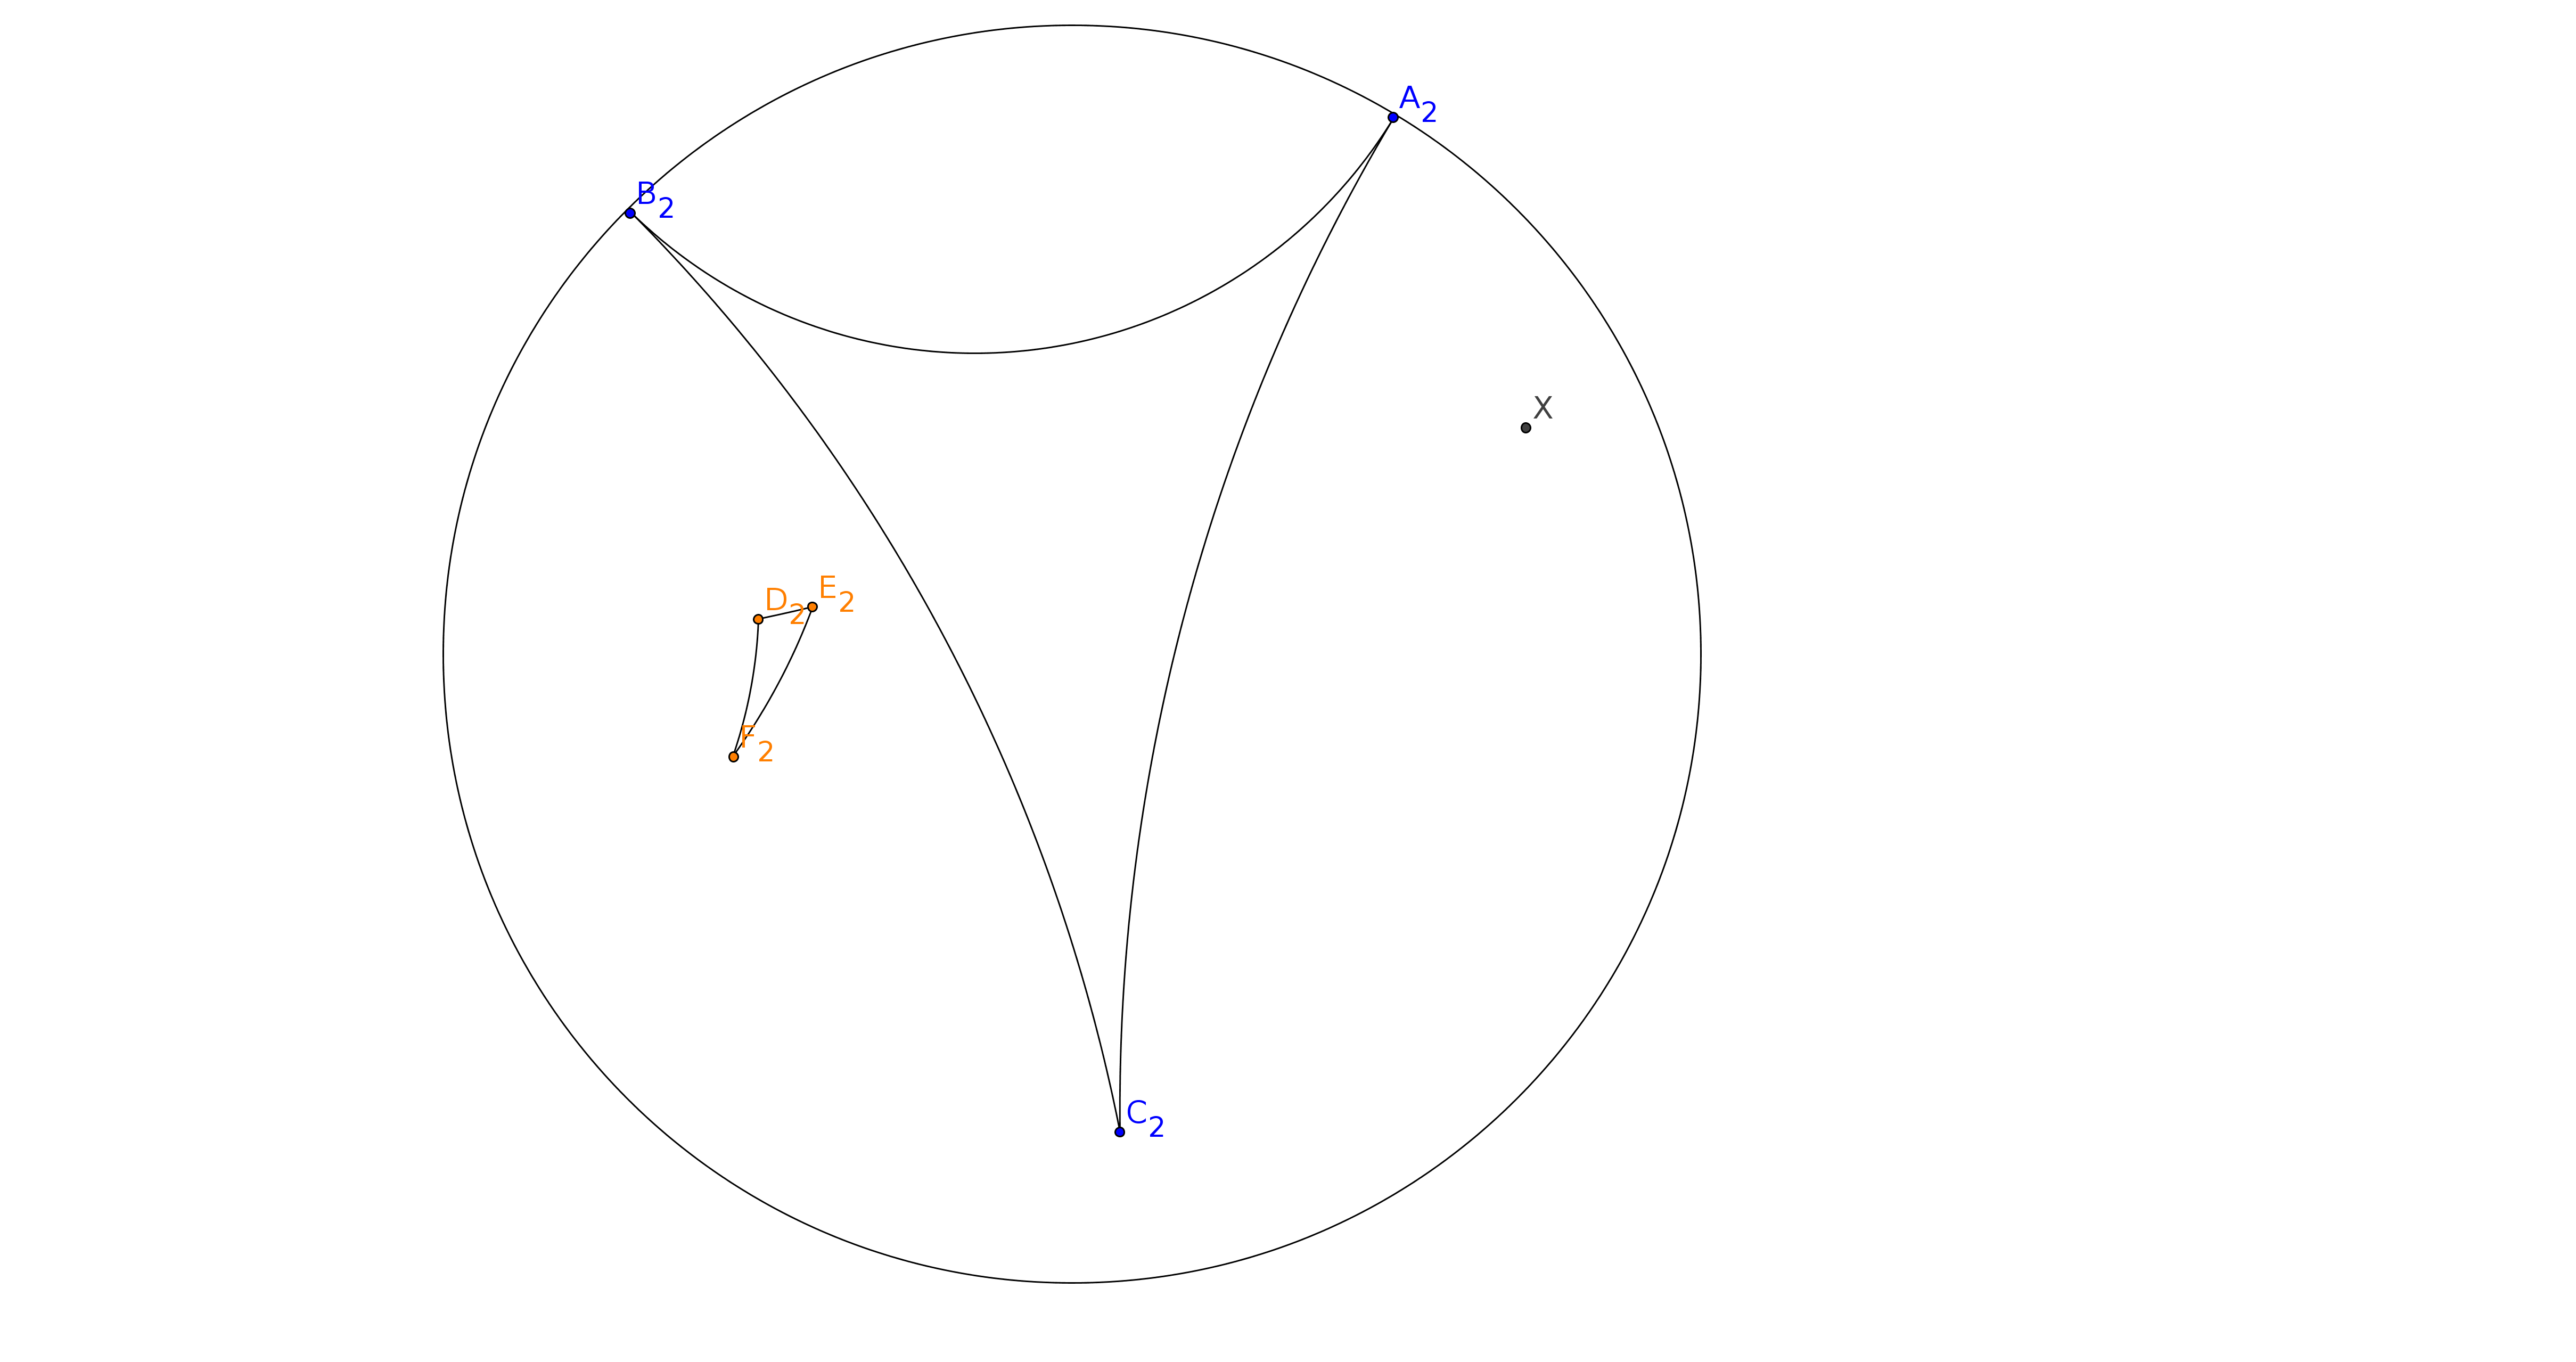
\includegraphics[width=65mm]{../images/triangle-2-point-reflection-2-1.png}\\
Triangle $T_2$ over point $X$ & Triangle $T_2$ over point $Y$  \\
\end{tabular}
\fi

From these diagrams we notice two oddities that we will discuss in turn. 

Firstly, these point reflections match an intuitive conception of a line reflection more than they do a point reflection. That is, the triangles seem to be ``reflected" and ``stretched" rather than ``rotated." However, a closer look at the matrix encodings of point reflections and line reflections sheds light on this. 

\wtftheorem{Theorem} All line reflections can be encoded as point reflections. 

\wtftheorem{Proof} Suppose that we have a line reflection $f_l$ given by $l = (l_1, l_2)$. Then, by WHATEVER WE CALL IT we encode the corresponding reflection in the matrix 
\[ M_l := \stanlinenoendmat. \]
To show that $f_l$ can be encoded as a point reflection, notice that 
\[ -1 \cdot \stanlinenoendmat = \lftmat{l_2}{l_1}{-1}{-l_2}.\]
Notice further that this matrix takes the form of a point reflection about $l = (l_1, l_2)$ if we take $\lambda = -1$. It follows that all line reflections can indeed be encoded as point reflections.
\wtfqed


More importantly, we now see that Guggenheimer's insistence that points be taken from the convex domain defined by the parabola $x = y^2$ (hereafter referred to simply as $E$) has no clear geometric motivation. Further, the examples in $\R$ demonstrate that this restriction is in fact entirely unnecessary. Consider Figure 2. We begin with a triangle $T_1$ defined by points contained in $D$. However, $T_1'$ (the result of reflecting $T_1$ over the point $(2, 1)$) is given by points that cannot be mapped from $D$ VERIFY AND REPHRASE. 

Further, 




%%%%%%%%%%%%%%%%%%%%%%%%%%%%%%%%%%%%%%%%%%%%%%%%%%%%%%
\newpage
%\wtftitle{Appendix A1: You wanna draw? Let's fuckin' draw!}
\wtftitle{Appendix A1: From $\R^2$ to the \poincare Disk}

Let $\Gamma$ be the \poincare disk. Suppose that we wish to translate the Euclidean point $A$, pictured arbitrarily below, to its equivalent point $A'$ in the \poincare disk.

\begin{center}
\begin{tikzpicture}[scale=.7]
\draw (0,0) circle (2.2cm) node[above left=1.5cm] {$\Gamma$};
\draw[fill=black] (2.2,2.2) circle (0.05) node[right] {$A$};
\end{tikzpicture}
\end{center}

We begin by constructing a line segment between $A$ and the origin $O$ and in order to find the Euclidean distance, $d_E$, between points $A$ and $O$.

\begin{center}
\begin{tikzpicture}[scale=.7]
\draw (0,0) circle (2.2cm) node[above left=1.5cm] {$\Gamma$};
\draw (0,0) -- (2.2,2.2);
\draw[fill=black] (0,0) circle (0.05) node[left] {$O$};
\draw[fill=black] (2.2,2.2) circle (0.05) node[right] {$A$};
\draw[decoration={brace,raise=4pt},decorate]
  (0,0) -- node[above left= 6pt] {$d_E$} (2.2,2.2);
\end{tikzpicture}
\end{center}

To construct the point $A'$, we want to find the radius $r$ in Euclidean distance of the circle whose hyperbolic distance from $O$ is $d_E$; $A'$ lies on this circle of radius $r$. In other words, if $d_H$ is the hyperbolic metric and $d_H(O,A') = d_E(O,A)$, then we want to find the circle, with radius $r\in\R$ centered at $O$, that contains $A'$. From \href{}{[source]} Theorem 9.1, we obtain the hyperbolic metric
\[
	d_H(O,A') = \ln\frac{1 + r}{1 - r}
\]
where $r\in\R$ is the radius of the circle we wish to draw. Let's call this new circle $\Delta$. Computing $r$, we find that
\[
	r = \frac{e^{d_H(O,A')} - 1}{e^{d_H(O,A')} + 1} =  \frac{e^{d_E(O,A)} - 1}{e^{d_E(O,A)} + 1}.
\]

\vfill
\pagebreak

Since $d_E(O,A)\in\R$, we conclude that $e^{d_E(O,A)} + 1 \neq 0$. Having computed $r$, we now draw the circle $\Delta$. 

\begin{center}
\begin{tikzpicture}[scale=.7]
\draw (0,0) circle (2.2cm) node[above left=1.5cm] {$\Gamma$};
\draw (0,0) circle (1.41cm) node[below right=.85cm] {$\Delta$};
\draw (0,0) -- (2.2,2.2);
\draw[fill=black] (0,0) circle (0.05) node[left] {$O$};
\draw[fill=black] (2.2,2.2) circle (0.05) node[right] {$A$};
\draw[fill=black] (1,1) circle (0.05) node[right] {$A'$};
\draw[decoration={brace,raise=4pt},decorate]
  (0,0) -- node[above left= 6pt] {$d_E$} (2.2,2.2);
\draw[decoration={brace,mirror,raise=4pt},decorate]
  (0,0) -- node[below right = 4pt] {$d_H$} (.95,.95);
\end{tikzpicture}
\end{center}

This point $A'$, the intersection between the line segment $\overline{OA}$ and $\Delta$, is the \poincare Disk-equivalent of our original point $A$.

%%%%%%%%%%%%%%%%%%%%%%%%%%% VI.preA %%%%%%%%%%%%%%%%%%%%%%%%%%%
\newpage 
\wtftitle{Appendix A2: Proof that $\fc$ Is a Field}

	Suppose $F$ is a field for which $-1$ is not the square of any number. The complexification of a field $F$ is the process of extending $F$ to a larger set by adding in the an element $i$ such that $i^2 = -1$ and then closing off under addition and multiplication. The resulting field, which we denote $F^\C$ is called the complexification of $F$ or the complexified field $F^\C$. One of the core example of complexification is the complexified reals $\R^\C$. As it turns out, this $\R^\C$ is the complex numbers $\C$. This can also be done to finite fields such as $\Z/3\Z$.

	Formally, recall that in order for $(F,+,\cdot)$ to be a field, it must satisfy the following axioms.
\begin{enumerate}
	\item $+$ must be associative and commutative.
	\item There exists an additive identity in $F$.
	\item Each $a\in F$ has an additive inverse.
	\item $\cdot$ must be associative and commutative.
	\item $+$ and $\cdot$ satisfy the distributive properties.
	\item There exists an multiplicative identity in $F$.
	\item Each $a\in F$ has an multiplicative inverse.
\end{enumerate}
Previously, all of the algebraic manipulations were carried out over a real ordered field in which all positive numbers have square roots. However, we may also carry out similar calculations over a complexified field. Let $(F,+,\cdot)$ be a field in which $-1$, the additive inverse of $1$, is not the square of any number in $F$. We define $F^\C = F\times F$. Further we define two new binary operations $\oplus$ and $\odot$ such that for all $(a,b)\ttc (c,d)\in F^\C$,
	\[
		(a,b)\oplus(c,d) = (a + c\ttc b + d)
	\]
and
	\[
		(a,b)\odot(c,d) = (ac - bd\ttc ad + bc).
	\]
wherein $+,-,\cdot$ are from $F$. We call $(F^\C,\oplus,\odot)$ the complexification of $F$. From hereon the rest of this section will be dedicated to proving the following theorem.

\begin{theorem}
	Let $(F,+,\cdot)$ be a field in which $-1$ is not a square. Then the complexification $(F^\C,\oplus,\odot)$ as defined above is a field.
\end{theorem}

\noindent First, let's resolve some properties of $\oplus$.\\

\begin{lemma}
	Given a complexification $(F^\C,\oplus,\odot)$, $\oplus$ is associative and commutative.
\end{lemma}

\begin{proof}

First we will show that $\oplus$ is associative. Let $(a,b)\ttc(c,d)\ttc(e,f)\in F^\C$.
\begin{align*}
	((a,b)\oplus(c,d))\oplus(e,f) & = (a + c\ttc b + d) + (e,f)\\
	& = ((a + c) + e\ttc (b + d) + f)\\
	& = (a + (c + e)\ttc b + (d + f)) & \text{(associativity of $+$)}\\
	& = (a,b) \oplus (c + e\ttc d + f)\\
	& = (a,b)\oplus ((c,d) \oplus (e,f))
\end{align*}
Hence $\oplus$ is associative. Now we argue that $\oplus$ is commutative. Let $(a,b)\ttc(c,d)\in F^\C$.
\begin{align*}
	(a,b)\oplus (c,d) & = (a + c\ttc b + d)\\
	& = (c + a\ttc d + b) & \text{(commutativity of $\oplus$)}\\
	& = (c,d)\oplus (a,b)
\end{align*}
Hence $\oplus$ is commutative. 
\end{proof}

Next, we argue that $F^\C$ has an additive identity.\\

\begin{lemma}
	The element $(0,0)\in F^\C$ is an additive identity.
\end{lemma}

\begin{proof}
Let $(a,b)\in F$ be arbitrary. We claim that $(0,0)\in F^\C$ is the additive identity of $F$. Using the fact that $0\in F$ is the additive identity, we obtain
	\[
		(a,b)\oplus (0,0) = (a + 0\ttc b + 0) = (a,b) = (0 + a\ttc, 0 + b) = (0,0) \oplus (a,b).
	\]
Therefore $(0,0)\in F^\C$ is an additive identity.
\end{proof} 

Since $F^\C$ has an additive identity, we may conjecture that $F^\C$ has additive inverses. 

\begin{lemma}
	For all $(x,y)\in F^\C$, there exists $(a,b)\in F^\C$ with 
	\[	
		(x,y)\oplus (a,b) = (0,0) = (a,b)\oplus (x,y).
	\]
	In other words, $F^\C$ has additive inverses.
\end{lemma}

\begin{proof}
Let $(a,b)\in F^\C$ be arbitrary. We claim that $(-a,-b)\in F^\C$ is the additive inverse of $(a,b)$. Note that since $F$ is a field, $-a\ttc -b$ exist and so $(-a,-b)\in F^\C$. Furthermore,
	\[
		(a,b)\oplus (-a,-b) = (a + -a\ttc b + -b) = (0,0) = (-a + a\ttc, -b + b) = (-a,-b) \oplus (a,b).
	\]
	Hence $\oplus$ is closed under inverses.
\end{proof}

Now we've proved that $\oplus$ has the desired properties that addition needs in a field. We therefore set our sights on resolving the properties of $\odot$.\\

\begin{lemma}
	The operation $\odot$ is associative and commutative.
\end{lemma}

\begin{proof}
	Now we argue via a similar line of reasoning that $\odot$ satisfies the properties of field multiplication. First we claim that $\odot$ is associative. Let $(a,b)\ttc(c,d)\ttc(e,f)\in F^\C$ be arbitrary. Using distributivity in $F$ and associativity and commutativity of $+$ and $\cdot$, we obtain
\begin{align*}
		((a,b)\odot(c,d))\odot(e,f) & = (ac - bd\ttc ad + bc)\odot (e,f)\\
		& = ((ac - bd)e - (ad + bc)f\ttc (ac - bd)f + (ad + bc)e)\\
		& = (ace - bde - adf - bcf\ttc acf - bdf + ade + bce)\\
		& = (a(ce - df) - b(de + cf)\ttc b(ce - df) + a(de + cf))\\
		& = (a,b)\odot (ce - df\ttc de + cf)\\
		& = (a,b)\odot ((c,d)\odot (e,f))
\end{align*}
Hence $\odot$ is associative. Now we show that $\odot$ is commutative. Let $(a,b)\ttc(c,d)\in F^\C$ be arbitrary. Then
	\begin{align*}
		(a,b)\odot (c,d) & = (ac - bd\ttc ad + bc)\\
		& = (ca - db\ttc da + cb) & \text{(commutativity of $\cdot$)}\\
		& = (c,d)\odot (a,b)
	\end{align*}
	Therefore $\odot$ is commutative.
\end{proof}

With these properties in mind, we now show that $F^\C$'s operations obey the distributive property.\\

\begin{lemma}
	The complexification $(F^\C,\oplus,\odot)$ obeys the distributive property.
\end{lemma}

\begin{proof}
Next we show that $F^\C$ has the distributive property. Let $(a,b)\ttc(c,d)\ttc(e,f)\in F^\C$ be arbitrary. Since $\odot$ is commutative, it suffices to argue that
	\[
		(a,b)\odot((c,d)\oplus(e,f)) = (a,b)\odot(c,d)\oplus(a,b)\odot(e,f).
	\]
	Following previous arguments, we find that
	\begin{align*}
		(a,b)\odot((c,d)\oplus(e,f)) & = (a,b)\odot(c + e\ttc d + f)\\
		& = (a(c + e) - b(d + f)\ttc a(d + f) + b(c + e))\\
		& = (ac + ae - bd - bf\ttc ad + af + bc + be) & \intertext{(distributivity in $F^\C$)}
		& = ((ac - bd) + (ae - bf)\ttc (ad + bc) + (af + be)) & \intertext{(commutativity and associativity of $+$)}
		& = (ac - bd\ttc ad + bc)\oplus (ae - bf\ttc af + be)\\
		& = (a,b)\odot (c,d)\oplus (a,b)\odot(e,f)
	\end{align*}
	Hence $F^\C$ has the distributive property. 
\end{proof}	

Since $F^\C$ satisfies the distributive property, we only have two properties left to demonstrate: multiplicative identities and multiplicative inverses. \\

\begin{lemma}
	The element $(1,0)\in F^\C$ is a multiplicative identity.
\end{lemma}

\begin{proof}
We claim that $(1,0)$ is the multiplicative identity of $F^\C$. Let $(a,b)\in F^\C$ be arbitrary. Note that since $F$ is a field, $1\in F$ is the multiplicative identity. Then
	\[
		(a,b)\odot(1,0) = (a\cdot 1 - b\cdot 0\ttc a\cdot 0 + b\cdot 1) = (a,b) = (1\cdot a - 0\cdot b\ttc 0\cdot a + 1\cdot b) = (1,0)\cdot (a,b).
	\]
	Hence $F^\C$ has a multiplicative identity.
\end{proof}

Since $F^\C$ has a multiplicative identity, we may conjecture that $F^\C$ has multiplicative inverses. \\
 
\begin{lemma}
	For all $(x,y)\in F^\C\backslash\{(0,0)\}$, there exists $(a,b)\in F^\C\backslash\{(0,0)\}$ with 
	\[	
		(x,y)\odot (a,b) = (1,0) = (a,b)\odot (x,y).
	\]
	In other words, $F^\C$ has multiplicative inverses.	
\end{lemma} 

\begin{proof}
Suppose $(a,b)\in F^\C\backslash\{(0,0)\}$. We hope to find $(x,y)\in F^\C$ with the property $(a,b)\odot(x,y) = (1,0)$. Since $\odot$ is commutative, this result holds for $(x,y)\odot(a,b)$ as well. Performing the multiplication, we find that
	\[
		(a,b)\odot(x,y) = (ax - by\ttc ay + bx) = (1,0)
	\]
	and so we obtain the equations
	\begin{align*}
		ax - by & = 1\\
		ay + bx & = 0
	\end{align*}
	Now we need to solve for $x$ and $y$. Multiply the upper equation by $a$ and the lower equation by $b$ to obtain
	\begin{align*}
		a^2x - aby & = a\\
		aby - b^2x & = 0
	\end{align*}
	Adding the two equations together, we find that
	\[
		x = \frac{a}{a^2 + b^2}.
	\]
	Via a similar process of multiplying the first equation by $b$ and the second equation by $a$ and adding the results, we also obtain
	\[
		y = \frac{-b}{a^2 + b^2}.
	\]
	Now we hope that there is no $(a,b)\in F^\C\backslash\{(0,0)\}$ with $a^2 + b^2 = 0$. Suppose such values do exist however. Since $(a,b)\neq (0,0)$, suppose $a\neq 0$. Then we conclude that
	\begin{align*}
		a^2 + b^2 = 0 & \text{ which implies } b^2 = -a^2\\
		& \text{ which implies } \frac{b^2}{a^2} = -1\\
		& \text{ which implies } \left(\frac{b}{a}\right)^2 = -1.
	\end{align*}
 	In other words, $-1$ is the square of $\frac{b}{a}\in F$, a contradiction since we assumed that no element in $F$ had $-1$ as its square. A similar argument can be made for when $b \neq 0$ using the fraction $\frac{a}{b}$. Hence $a^2 + b^2 \neq 0$ for any $(a,b)\in F^\C\backslash\{(0,0)\}$. Therefore $F^\C$ has multiplicative inverses.
\end{proof} 	
 	
Combining these seven lemmas, we conclude that $(F^\C,\oplus,\odot)$ is a field as desired. Hence the theorem is true and so the complexification of a field is a field. 





%%%%%%%%%%%%%%%%%%%%%%%%%%% I.A %%%%%%%%%%%%%%%%%%%%%%%%%%%
\newpage
\wtftitle{Appendix A4: Coode}

Below is the code we used to apply point reflections and line reflections to various points. 

\noindent[here we will cahpy-past our coode]






\iffalse
%%%%%%%%%%%%%%%%%%%%%%%%%%% I.A %%%%%%%%%%%%%%%%%%%%%%%%%%%
\newpage
\wtftitle{Appendix A3: Do we actually need this...?}

\noindent Define the group
	\[
		A = \left\lbrace z\mapsto \frac{az + b}{cz + d}\colon a,b,c,d\in F\text{ with } ad - bc \neq 0\right\rbrace
	\]
of linear fractional transformations and let $GL_2(F)$ denote the group of invertible $2\times 2$ matrices with entries in $F$. Also define the subset
	\[
		F^* = \left\lbrace\lftmat{\lambda}{0}{0}{\lambda}\colon \lambda\in F\text{ with } \lambda\neq 0 \right\rbrace.
	\]
	We argue that $F^*$ is a normal subgroup of $GL_2(F)$.\footnote{Insert math here} With this in mind, we now define the map $\varphi\colon A\rightarrow GL_2(F)/F^*$ by
	\[
		\varphi\left(z\mapsto \frac{az + b}{cz + d}\right) = \stanlftmat F^*
	\]
	We claim that $\varphi$ is a homomorphism. \footnote{Insert more math here}Now that we've established that $\varphi$ is a homomorphism, we now argue that $\varphi$ is surjective. \footnote{And a little bit more right here}  Next we identify the kernel of $\varphi$ in order to establish an isomorphism between $A/\ker(\varphi)$ and $GL_2(F)/F^*$\footnote{Technically we don't need the kernel to identify the isomorphism; it's just noteworthy and tells us when we can't recover a linear fractional transformation.}. Finally by the First Isomorphism Theorem, we conclude that $A/\ker(\varphi)$\footnote{insert whatever the kernel turns out to be here} is isomorphic to $GL_2(F)/F^*$. 
\fi
	









%%%%%%%%%%%%%%%%%%%%%%%%%%% I.A %%%%%%%%%%%%%%%%%%%%%%%%%%%
\newpage
\wtftitle{``Bibliography" (List of Sources)} 

\begin{enumerate}
	\item http://people.reed.edu/mayer/math112.html/chap04.pdf (Complexification of a Field)
	\item H. Guggenheimer, Plane Geometry and Its Groups, Holden-Day San Francisco (now Kreiger, Huntington N.Y.), 1967, Chap, 9.
	\item Guggenheimer's paper itself
	\item Robin Hartshorne, Geometry: Euclid And Beyond, Srpinger-Verlag New York, 2000, Chap, 7.
	\item https://www.geogebra.org/material/show/id/7005
	\item https://www.geogebra.org/home
\end{enumerate}


%https://tex.stackexchange.com/questions/16617/use-tikz-for-example-to-draw-pictures-in-hyperbolic-geometry
% https://tex.stackexchange.com/questions/61316/draw-a-plot-with-point
% https://tex.stackexchange.com/questions/230566/making-curly-braces-with-tikz
%http://www.ms.uky.edu/~droyster/courses/spring08/math6118/Classnotes/Chapter09.pdf







\end{document}